\documentclass[aspectratio=169]{beamer}
\usepackage{tikz}
\usetikzlibrary{arrows,shapes}
\tikzstyle{vertex}=[circle,fill=black!25,minimum size=10pt,inner sep=0pt]
\tikzstyle{blue vertex}=[circle,fill=blue!100,minimum size=10pt,inner sep=0pt]
\tikzstyle{red vertex}=[circle,fill=red!100,minimum size=10pt,inner sep=0pt]
%\tikzstyle{label}=[thin, draw=black, align=center,minimum width=0.5cm, minimum height=0.5cm,fill=white]
\tikzstyle{edge} = [draw,thick,-]
\tikzstyle{red edge} = [draw, line width=5pt,-,red!50]
\tikzstyle{black edge} = [draw, line width=5pt,-,black!20]
\tikzstyle{weight} = [font=\smaller]


\usepackage{amssymb,amsmath}
\usepackage{graphicx}
\usepackage{url}
\usepackage{color}
\usepackage{relsize}		% For \smaller
\usepackage{url}			% For \url
\usepackage{epstopdf}	% Included EPS files automatically converted to PDF to include with pdflatex
\usepackage{pagenote}[continuous,page]

%For MindMaps
% \usepackage{tikz}%
% \usetikzlibrary{mindmap,trees,arrows}%

%%% Color Definitions %%%%%%%%%%%%%%%%%%%%%%%%%%%%%%%%%%%%%%%%%%%%%%%%%%%%%%%%%
%\definecolor{bordercol}{RGB}{40,40,40}
%\definecolor{headercol1}{RGB}{186,215,230}
%\definecolor{headercol2}{RGB}{80,80,80}
%\definecolor{headerfontcol}{RGB}{0,0,0}
%\definecolor{boxcolor}{RGB}{186,215,230}

%%% Save space in lists. Use this after the opening of the list %%%%%%%%%%%%%%%%
%\newcommand{\compresslist}{
%	\setlength{\itemsep}{1pt}
%	\setlength{\parskip}{0pt}
%	\setlength{\parsep}{0pt}
%}

%\setbeameroption{show notes on top}

% You should run 'pdflatex' TWICE, because of TOC issues.

% Rename this file.  A common temptation for first-time slide makers
% is to name it something like ``my_talk.tex'' or
% ``john_doe_talk.tex'' or even ``discrete_math_seminar_talk.tex''.
% You really won't like any of these titles the second time you give a
% talk.  Try naming your tex file something more descriptive, like
% ``riemann_hypothesis_short_proof_talk.tex''.  Even better (in case
% you recycle 99% of a talk, but still want to change a little, and
% retain copies of each), how about
% ``riemann_hypothesis_short_proof_MIT-Colloquium.2000-01-01.tex''?

\mode<presentation>
{
  % A tip: pick a theme you like first, and THEN modify the color theme, and then add math content.
  % Warsaw is the theme selected by default in Beamer's installation sample files.

  %%%%%%%%%%%%%%%%%%%%%%%%%%%% THEME
  %\usetheme{Madrid}		% No subsection
  \usetheme{AnnArbor}  % Subsection on top, no color


  %\usetheme{Antibes}
  %\usetheme{Bergen}
  %\usetheme{Berkeley}		% bem bacana - menu esquerdo
  %\usetheme{Berlin}
  %\usetheme{Boadilla}
  %\usetheme{boxes}
  %\usetheme{CambridgeUS}		% bem bacana - menu superior
  %\usetheme{Copenhagen}
  %\usetheme{Darmstadt}
  %\usetheme{default}
  %\usetheme{Dresden}
  %\usetheme{Frankfurt}
  %\usetheme{Goettingen}
  %\usetheme{Hannover}		% bem bacana - menu esquerdo
  %\usetheme{Ilmenau}
  %\usetheme{JuanLesPins}
  %\usetheme{Luebeck}
  %\usetheme{Malmoe}
  %\usetheme{Marburg}		% bem bacana - menu direito
  %\usetheme{Montpellier}
  %\usetheme{PaloAlto}		% bem bacana - menu esquerdo
  %\usetheme{Pittsburgh}
  %\usetheme{Rochester}		%bacana
  %\usetheme{Singapore}
  %\usetheme{Szeged}
  %\usetheme{Warsaw}

  %%%%%%%%%%%%%%%%%%%%%%%%%%%% COLOR THEME
  %\usecolortheme{default}		% branco, azul clarinho
  \usecolortheme{crane}		% Very yellow (ok)

  %\usecolortheme{albatross}		% azul escuro, massa
  %\usecolortheme{beetle}		% cinza, menu azul
  %\usecolortheme{dolphin}		% azul e branco, legal
  %\usecolortheme{dove}			% cinza e branco, feio
  %\usecolortheme{fly}			% todo cinza, horrível
  %\usecolortheme{lily}			% parece o default
  %\usecolortheme{orchid}		% azul e branco, ok
  %\usecolortheme{rose}			% branco e violeta-claro, bonito
  %\usecolortheme{seagull}		% cinza, feio
  %\usecolortheme{seahorse}		% nhé, meio feio
  %\usecolortheme{sidebartab}		% Azul, branco, destaque na tab, interessante
  %\usecolortheme{structure}		% bichado
  %\usecolortheme{whale}		% Azul e branco, bem bonito

  %%%%%%%%%%%%%%%%%%%%%%%%%%%% OUTER THEME
  \useoutertheme{default}
  %\useoutertheme{infolines}
  %\useoutertheme{miniframes}
  %\useoutertheme{shadow}
  %\useoutertheme{sidebar}
  %\useoutertheme{smoothbars}
  %\useoutertheme{smoothtree}
  %\useoutertheme{split}
  %\useoutertheme{tree}

  %%%%%%%%%%%%%%%%%%%%%%%%%%%% INNER THEME
  \useinnertheme{circles}
  %\useinnertheme{default}
  %\useinnertheme{inmargin}
  %\useinnertheme{rectangles}
  %\useinnertheme{rounded}

  %%%%%%%%%%%%%%%%%%%%%%%%%%%%%%%%%%%

  \setbeamercovered{invisible} % or whatever (possibly just delete it)
  % To change behavior of \uncover from graying out to totally
  % invisible, can change \setbeamercovered to invisible instead of
  % transparent. apparently there are also 'dynamic' modes that make
  % the amount of graying depend on how long it'll take until the
  % thing is uncovered.

}


% Get rid of nav bar
\beamertemplatenavigationsymbolsempty

% Use short top
%\usepackage[headheight=12pt,footheight=12pt]{beamerthemeboxes}
%\addheadboxtemplate{\color{black}}{
%\hskip0.5cm
%\color{white}
%\insertshortauthor \ \ \ \
%\insertframenumber \ \ \ \ \ \ \
%\insertsection \ \ \ \ \ \ \ \ \ \ \ \ \ \ \ \ \  \insertsubsection
%\hskip0.5cm}
%\addheadboxtemplate{\color{black}}{
%\color{white}
%\ \ \ \
%\insertsection
%}
%\addheadboxtemplate{\color{black}}{
%\color{white}
%\ \ \ \
%\insertsubsection
%}

% Insert frame number at bottom of the page.
% \usefoottemplate{\hfil\tiny{\color{black!90}\insertframenumber}}

%% makes the ppagenote command for figure references at the end.

\usepackage[english]{babel}
%qq\usepackage[latin1]{inputenc}
\usepackage{CJKutf8}
\usepackage{subfigure}

\usepackage{times}
\usepackage[T1]{fontenc}

\makepagenote
\renewcommand{\notenumintext}[1]{}
\newcommand{\ppagenote}[1]{\pagenote[Page \insertframenumber]{#1}}

\title[Programming Challenges]{GB20602 - Programming Challenges}
\author[Claus Aranha]{Claus Aranha\\{\footnotesize caranha@cs.tsukuba.ac.jp}}
\institute[U. Tsukuba]{University of Tsukuba, Department of Computer Sciences}


\subtitle[Week 5: Graph I]{Week 5 - Graph Part I: Basics}
\date[]{{\smaller(last updated: \today)}}

\begin{document}
\begin{CJK}{UTF8}{ipxm}

\begin{frame}
\maketitle
\vfill

\hfill Version 2022
\end{frame}



\section{Introduction}

\begin{frame}
  \frametitle{Computational Geometry}
  \framesubtitle{What is it?}

  {\small

    \structure{Computational Geometry} problems involve answering
    questions about \structure{lines, points and angles}. Some example
    questions:

    \bigskip

    \begin{block}{}
    \only<1>{Given $N$ points $(s_1, s_2, s_3, \ldots, s_N)$, what is
      the area of the poligon that covers all the points?}

    \only<2>{Given $N$ rectangles, $x_1,y_1,w_1,h_1; \ldots; x_N, y_N,
      w_N, h_N$, what is the length of lines needed to connect them?}

    \only<3>{Given a polygon, and $N$ points, what is the line
      that divides the polygon in equal areas, so that the same
      number of points are in each area?}
    \end{block}

    \begin{center}
      \includegraphics<1>[width=0.8\textwidth]{img/sampleproblem_1.png}
      \includegraphics<2>[width=0.6\textwidth]{img/sampleproblem_2.png}
      \includegraphics<3>[width=0.4\textwidth]{img/sampleproblem_3.png}
    \end{center}

  }
\end{frame}

\begin{frame}
  \frametitle{Computational Geometry}
  \framesubtitle{The good and the bad}

  \begin{itemize}
  \item \structure{Good}: Geometry problems are fun
  \item \structure{Good}: You have to draw pretty pictures
  \item \structure{Good}: Mostly algorithms from high school
  \item \structure{Good}: Code is highly re-usable

    \bigskip

  \item \alert{Bad}: You have to write a lot of code (in the beginning!)
  \item \alert{Bad}: Very easy to get WE...
  \end{itemize}
\end{frame}


\begin{frame}
  \frametitle{Easy Mistakes in Geometry Problems}

  {\small
    \begin{block}{Problem 1 -- Special Cases}
      \begin{itemize}
      \item Multiple points in the same place;
      \item Collinear points;
      \item Vertical lines;
      \item Parallel Lines;
      \item Intersection at end of segment;
      \item etc;
      \end{itemize}
    \end{block}

    \begin{block}{Problem 2 -- Precision Errors}
      \begin{itemize}
      \item Functions require many multiplications and divisions;
      \item Easy to propagate floating point errors;
      \end{itemize}
    \end{block}
  }
\end{frame}


\begin{frame}[fragile]
  \frametitle{Easy Mistakes in Geometry Problems}

  {\smaller

    \begin{block}{Dealing Special Cases}
      \begin{itemize}
      \item Make sure to add special cases to your
        library functions;
      \end{itemize}
    \end{block}

    \begin{block}{Solving Precision Errors}
      \begin{itemize}
      \item If possible, convert all values to integers
      \item Use an EPSILON constant for comparisons:

\begin{verbatim}
if (float.1 == float.2) then            // NO
if (fabs(float.1 - float.2) < EPS) then // YES!
\end{verbatim}

      \end{itemize}
    \end{block}
  }
\end{frame}

\begin{frame}
  \frametitle{Class Outline}
  \begin{itemize}
  \item Example Problems;
  \item Basic Geometric Functions;
  \item Circles;
  \item Triangles;
  \item Polygons;
  \end{itemize}
\end{frame}


\section{Common Graph Problems}

\begin{frame}{}
  \begin{center}
    {\bf Part II: Common Graph Problems}
  \end{center}
\end{frame}

\begin{frame}{Common Graph Problems in Competitive Programming}

  Let's see some common problems that can be solved using DFS or BFS.\bigskip

  \begin{itemize}
    \item Connected Components;
    \item Flood Fill;
    \item Topological Sort;
    \item Bipartite Checking;
  \end{itemize}
\end{frame}


\subsection{Connected Components}
\begin{frame}{Connected Components (undirected graph)}
  A {\bf connected component} of a graph is a subset of vertices $C \subset V$ where every pair of vertices $v_i, v_j \in C$ is connected.\bigskip

  The graph below has 3 connected components (abcd, e, fg)\bigskip


  \vfill
  \begin{center}
    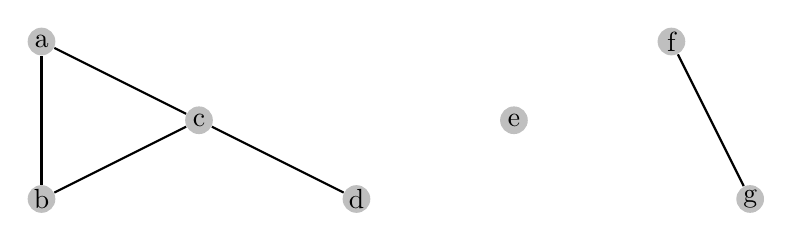
\begin{tikzpicture}[scale=1,auto,swap]
      \node[vertex] (a) at (0,2) {a};
      \node[vertex] (b) at (0,0) {b};
      \node[vertex] (c) at (2,1) {c};
      \node[vertex] (d) at (4,0) {d};
      \node[vertex] (e) at (6,1) {e};
      \node[vertex] (f) at (8,2) {f};
      \node[vertex] (g) at (9,0) {g};
      \draw[edge] (a) to (b);
      \draw[edge] (b) to (c);
      \draw[edge] (c) to (a);
      \draw[edge] (c) to (d);
      \draw[edge] (f) to (g);
    \end{tikzpicture}
  \end{center}
\end{frame}

\begin{frame}{Connected Components}
  \begin{block}{Problem Example: Extra cables}
    There is a network of $N$ computers. Some of the computers are connected by cables. Computers connected by cables, even if indirectly, are said to be on the {\bf same network}.
    \bigskip

    What is the minimum number of cables that you need to make sure that all $N$ computers are part of the same network?
  \end{block}\bigskip

  {\bf Solution:} Count the number of Connected Components ($C$), the answer is $C-1$.\bigskip

  {\bf Quiz:} How do you implement this?
\end{frame}

\begin{frame}[fragile]{Connected Components}{Finding Connected Components using BFS/DFS}
  We can find all connected components by looping through all vertices, and running BFS/DFS on each unvisited vertice;

\begin{columns}
  \column{0.7\textwidth}
  \begin{exampleblock}{}
\begin{verbatim}
int dfs_vis[];          // visited vertices

int cables = 0;
for (int = 0; i < N; i++)
   if (dfs_vis[i] == 0) // found new component
   {
      dfs(i);           // visit more vertices
      cables += 1;
   }
cout << "Need "<< cables - 1 <<".\n";
\end{verbatim}
  \end{exampleblock}
  \column{0.3\textwidth}
  \begin{center}
  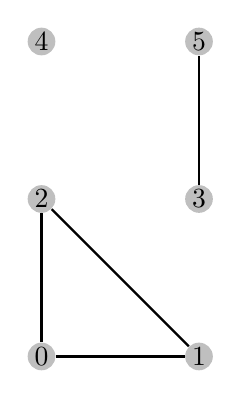
\begin{tikzpicture}[scale=1,auto,swap]
    \node[vertex] (a) at (0,0) {0};
    \node[vertex] (b) at (2,0) {1};
    \node[vertex] (c) at (0,2) {2};
    \node[vertex] (d) at (2,2) {3};
    \node[vertex] (e) at (0,4) {4};
    \node[vertex] (f) at (2,4) {5};
    \draw[edge] (a) to (b);
    \draw[edge] (a) to (c);
    \draw[edge] (b) to (c);
    \draw[edge] (d) to (f);
  \end{tikzpicture}
\end{center}
\end{columns}

\end{frame}

%% Maybe add back later
% \begin{frame}[fragile]{Connected Components}{UFDS Variant}
%
%   You could also count Connected Components using the {\bf UFDS} data structure from lecture 2.\bigskip
%
%   It costs $O(E)$ to build the UFDS, and $O(V)$ to count the number of components.\bigskip
%
%   If your problem is dynamic and includes several additions to the graph edges, this might be a good choice, because it is cheaper to recalculate the CCs.
% \end{frame}

\subsection{Flood Fill}

\begin{frame}[fragile]{Flood Fill}
  \begin{block}{Problem: Find The Biggest Island}
    You want to find the biggest island in a game map to build a castle.

    {\bf Input:} A 2D representation of the map:
\begin{verbatim}
....................................
.###.......###.....#.....###.####...
.#####....#####.##.#####.##....#....
.###........###..#...##..#....###...
......###.......###...####...##.....
....####.............######.....###.
....####.......#.......###......###.
....................................
\end{verbatim}
  \end{block}
  \hfill Can we solve this as a graph problem?
\end{frame}

\begin{frame}{Implicit Graphs}
  \begin{columns}
    \column{0.7\textwidth}
    \begin{itemize}
      \item {\bf Implict Graphs} are data that suggest graph organization. Examples:
      \begin{itemize}
        \item grids (NSWE connections)
        \item maps (distance = weights)
      \end{itemize}\bigskip

      \item In some problems, it is not necessary to store the entire graph from the beginning;\bigskip

      \item {\bf Grid Floodfill}: Painting images, Walkable tiles in videogames, etc;
      \item Algorithm is just BFS/DFS with vertex labels;
    \end{itemize}
    \column{0.3\textwidth}
    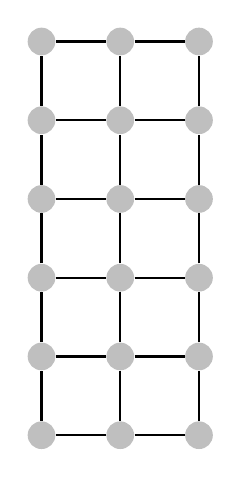
\begin{tikzpicture}[scale=1,auto,swap]
      \node[vertex] (00) at (0,0) {};
      \node[vertex] (01) at (0,1) {};
      \node[vertex] (02) at (0,2) {};
      \node[vertex] (03) at (0,3) {};
      \node[vertex] (04) at (0,4) {};
      \node[vertex] (05) at (0,5) {};
      \node[vertex] (10) at (1,0) {};
      \node[vertex] (11) at (1,1) {};
      \node[vertex] (12) at (1,2) {};
      \node[vertex] (13) at (1,3) {};
      \node[vertex] (14) at (1,4) {};
      \node[vertex] (15) at (1,5) {};
      \node[vertex] (20) at (2,0) {};
      \node[vertex] (21) at (2,1) {};
      \node[vertex] (22) at (2,2) {};
      \node[vertex] (23) at (2,3) {};
      \node[vertex] (24) at (2,4) {};
      \node[vertex] (25) at (2,5) {};
      \draw[edge] (00) to (01);\draw[edge] (00) to (10);
      \draw[edge] (01) to (02);\draw[edge] (01) to (11);
      \draw[edge] (02) to (03);\draw[edge] (02) to (12);
      \draw[edge] (03) to (04);\draw[edge] (03) to (13);
      \draw[edge] (04) to (05);\draw[edge] (04) to (14);
      \draw[edge] (10) to (11);\draw[edge] (10) to (20);
      \draw[edge] (11) to (12);\draw[edge] (11) to (21);
      \draw[edge] (12) to (13);\draw[edge] (12) to (22);
      \draw[edge] (13) to (14);\draw[edge] (13) to (23);
      \draw[edge] (14) to (15);\draw[edge] (14) to (24);
      \draw[edge] (20) to (21);\draw[edge] (21) to (22);
      \draw[edge] (22) to (23);\draw[edge] (23) to (24);
      \draw[edge] (24) to (25);\draw[edge] (15) to (25);
      \draw[edge] (05) to (15);
    \end{tikzpicture}
  \end{columns}

\end{frame}


\begin{frame}[fragile]{Flood Fill}{Finding the "Biggest Island" with BFS/DFS and modifying labels}

  {\smaller
  \begin{exampleblock}{}
\begin{verbatim}
int dr[] = {1,1,0,-1,-1,-1,0,1}; // neighbors for a grid
int dc[] = {0,1,1,1,0,-1,-1,-1}; // with diagonals;

int floodfill(int y, int x) {    // size of one position
  if (y < 0 || y >= R || x < 0 || x >= C) return 0;
  if (grid[y][x] != '#') return 0;
  int size = 1;
  grid[y][x] = '.';              // Change the map to mark visited nodes
  for (int d = 0; d < 8; d++)
     size += floodfill(y+dr[d], x+dc[d]);
  return ans;
}
biggest = 0;
for (int i = 0; i < C; i++)
  for (int j = 0; j < R; j++)
    biggest = max(biggest, floodfill(i,j));
\end{verbatim}
  \end{exampleblock}
  }
\end{frame}

\subsection{Topological Sort}

\begin{frame}[fragile]{Topological Sort}
  \begin{block}{Example Problem: Preparing a Curriculum}
    You have a list of courses and requisites.\\
    Choose an {\bf ordering} of topics that respect all requisites.
    \bigskip

    {\bf Input}: list M topics, and N pairs of topics;\\
    {\bf Output}: Sorted list of all topics;
  \end{block}

{\smaller
\begin{verbatim}
** Example Input:
5 4 Graphs DP Search Flow Programming
Programming -> Search
Search -> DP
Graph -> Flow
Search -> Graph

** Example Output:
Course: Programming -> Search -> DP -> Graph -> Flow
\end{verbatim}

  }
\end{frame}

\begin{frame}{Topological Sort Definition}
  A {\bf topological sort} is an ordering of vertices where $v_i \prec v_j$ only if there is no path $v_j \to v_i$.\bigskip
  \begin{center}
    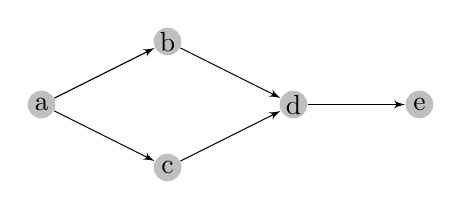
\begin{tikzpicture}[scale=.8,auto,swap]
  \node[vertex] (a) at (0,0) {a};
  \node[vertex] (b) at (2,1) {b};
  \node[vertex] (c) at (2,-1) {c};
  \node[vertex] (d) at (4,0) {d};
  \node[vertex] (e) at (6,0) {e};
  \tikzset{edge/.style = {->,>=latex'}}
  \draw[edge] (a) to (b);
  \draw[edge] (a) to (c);
  \draw[edge] (c) to (d);
  \draw[edge] (b) to (d);
  \draw[edge] (d) to (e);
\end{tikzpicture}

  \end{center}
  For this graph, one possible topological sort is $a \prec b \prec c \prec d \prec e$.\bigskip

  \begin{itemize}
    \item Toposorts are {\bf not unique}:
    \begin{itemize}
      \item $a \prec c \prec b \prec d \prec e$ is also a toposort.
    \end{itemize}
    \item A graph only has a toposort if it has {\bf no cycles}.
    \item To find the toposort, we use {\bf in-degrees and out-degrees} of each vertex:
    \begin{itemize}
      \item $a$ -- In-deg: 0; Out-deg: 2;
      \item $d$ -- In-deg: 2; Out-deg: 1;
      \item $e$ -- In-deg: 1; Out-deg: 0;
    \end{itemize}
  \end{itemize}
\end{frame}

\begin{frame}[fragile]{Finding Topological Sort -- Khan's Algorithm}

Modified BFS: Vertices are only added to the queue if they in-degree is 0.

\begin{exampleblock}{}
  {\smaller
\begin{verbatim}
queue<int> q; vector<int> toposort;
vector<int> in-deg;                 // initialize to 0 for all N;

for (int i = 0; i < EdgeList.size(); i++)
  in-deg[EdgeList[i].second]++;     // calculate in-degrees based on edge list.
for (int i = 0; i < N; i++)
  if (in-deg[i] == 0) q.push(i);    // add vertices with in-deg = 0 to queue

while (!q.empty()) {
  u = q.front(); q.pop(); toposort.push_back(u); // Add top of queue to toposort
  for (int i = 0; i < EdgeList[u].size(); i++) {
    d = EdgeList[u][i].first; in-deg[d]--;       // remove edges from visited.
    if (in-deg[d] == 0) q.push(d); // queue in-deg = 0;
  }
}
\end{verbatim}}
  \end{exampleblock}
\end{frame}

\begin{frame}{Khan's Algorithm}{Simulation}
  \begin{center}
    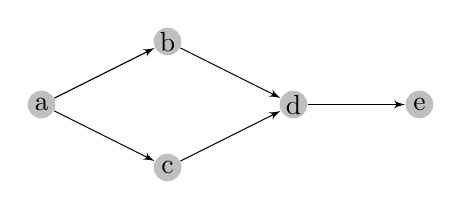
\begin{tikzpicture}[scale=.8,auto,swap]
  \node[vertex] (a) at (0,0) {a};
  \node[vertex] (b) at (2,1) {b};
  \node[vertex] (c) at (2,-1) {c};
  \node[vertex] (d) at (4,0) {d};
  \node[vertex] (e) at (6,0) {e};
  \tikzset{edge/.style = {->,>=latex'}}
  \draw[edge] (a) to (b);
  \draw[edge] (a) to (c);
  \draw[edge] (c) to (d);
  \draw[edge] (b) to (d);
  \draw[edge] (d) to (e);
\end{tikzpicture}

  \end{center}
  {\bf In-deg list:}
  \begin{itemize}
    \item<2-> iteration 1: (a,0), (b,1), (c,1), (d,2), (e,1)\hfill visit a
    \item<3-> iteration 2: (b,0), (c,0), (d,2), (e,1)\hfill visit b
    \item<4-> iteration 3: (c,0), (d,1), (e,1), \hfill visit c
    \item<5-> iteration 4: (d,0), (e,1)\hfill visit d
    \item<6-> iteration 5: (e,0)\hfill visit e
  \end{itemize}
  {\bf Toposort: \only<2->{a,} \only<3->{b,} \only<4->{c,} \only<5->{d,} \only<6->{e}}
\end{frame}

% \begin{frame}
%   \frametitle{Topological Sort and Bottom-Up Dynamic Programming}
%
%   %TODO
%   What is the relationship between Topological Sort and Bottom-up DP?
%
%   \bigskip
%
%   Bottom-up DP are Topological sorts on Tables!
% \end{frame}

\subsection{Bipartite Checking}
\begin{frame}{Bipartite Graphs}{Definition}
  \begin{columns}
    \column{.7\textwidth}
      Intuitively, a {\bf Bipartite Graph} is one that we can separate between a "left" side and a "right" side.\bigskip

      More generally, a graph $(V,E)$ is bipartite if you can completely partition its vertices in two subsets: $V_1$ and $V_2$, so that {\bf there are no edges} connecting two vertices in the same subset.\bigskip

      Bipartite graphs appear in a large number of algorithms. In particular, {\bf flow graphs} (next week) are bipartite graphs.\bigskip

      Most neural networks are bipartite graphs too!\\
      {\bf Quiz:} How do you test if a graph is bipartite?
    \column{.3\textwidth}
    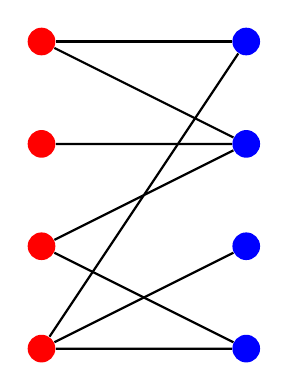
\begin{tikzpicture}[scale=1.3,auto,swap]
  \node[red vertex] (a) at (0,0) {};
  \node[blue vertex] (b) at (2,0) {};
  \node[blue vertex] (c) at (2,-1) {};
  \node[red vertex] (d) at (0,-1) {};
  \node[red vertex] (e) at (0,-2) {};
  \node[red vertex] (f) at (0,-3) {};
  \node[blue vertex] (g) at (2,-2) {};
  \node[blue vertex] (h) at (2,-3) {};
  \draw[edge] (a) to (b);
  \draw[edge] (a) to (c);
  \draw[edge] (b) to (f);
  \draw[edge] (c) to (d);
  \draw[edge] (c) to (e);
  \draw[edge] (f) to (h);
  \draw[edge] (e) to (h);
  \draw[edge] (f) to (g);
\end{tikzpicture}

  \end{columns}
\end{frame}

\begin{frame}[fragile]
  \frametitle{Bipartite Check Algorithm}
  Visit all vertices using BFS/DFS. Every time we visit a vertice, we mark it "0" or "1". If two adjacent vertices are of the same colors, the graph is not bipartite.

  {\smaller
  \begin{exampleblock}{}
\begin{verbatim}
queue<int> q; q.push(s);
vector<int> color(V, -1); color[s] = 0; // Starting vertex
bool isBipartite = True;

while (!q.empty() && isBipartite) {
   int u = q.front(); q.pop();
   for (int j=0; j < adj_list[u].size(); j++) {
      v = adj_list[u][j].first;
      if (color[v] == -1) {
         color[v] = 1 - color[i];        // Coloring new vertex
         q.push(v.first);}
      else if (color[v.first] == color[u]) {
         isBipartite = False;            // Bipartite collision
}}}
\end{verbatim}
  \end{exampleblock}
  }
\end{frame}

\begin{frame}
  \frametitle{Bipartite Check -- Visualization}
  \begin{columns}[t]
    \column{0.5\textwidth}
    \begin{exampleblock}{Testing Bipartite property}
      \vspace{0.1cm}
      \begin{center}
        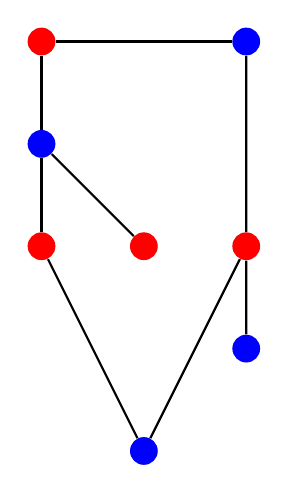
\begin{tikzpicture}[scale=1.3,auto,swap]
          \node[vertex] (a) at (0,0) {};
          \node[vertex] (b) at (2,0) {};
          \node[vertex] (c) at (0,-1) {};
          \node[vertex] (d) at (1,-2) {};
          \node[vertex] (e) at (0,-2) {};
          \node[vertex] (f) at (2,-2) {};
          \node[vertex] (g) at (2,-3) {};
          \node[vertex] (h) at (1,-4) {};
          \draw[edge] (a) to (b);
          \draw[edge] (a) to (c);
          \draw[edge] (b) to (f);
          \draw[edge] (c) to (d);
          \draw[edge] (c) to (e);
          \draw[edge] (f) to (h);
          \draw[edge] (e) to (h);
          \draw[edge] (f) to (g);
          \uncover<2->{\node[red vertex] (a1) at (0,0) {};}
          \uncover<3->{\node[blue vertex] (b1) at (2,0) {};}
          \uncover<3->{\node[blue vertex] (c1) at (0,-1) {};}
          \uncover<4->{\node[red vertex] (d1) at (1,-2) {};}
          \uncover<4->{\node[red vertex] (e1) at (0,-2) {};}
          \uncover<4->{\node[red vertex] (f1) at (2,-2) {};}
          \uncover<5->{\node[blue vertex] (g1) at (2,-3) {};}
          \uncover<5->{\node[blue vertex] (h1) at (1,-4) {};}
        \end{tikzpicture}
      \end{center}
      \vspace{0.1cm}
    \end{exampleblock}
    \column{0.5\textwidth}
    \uncover<6->{
    \begin{exampleblock}{Rearranging the nodes}
      \vspace{0.1cm}
      \begin{center}
        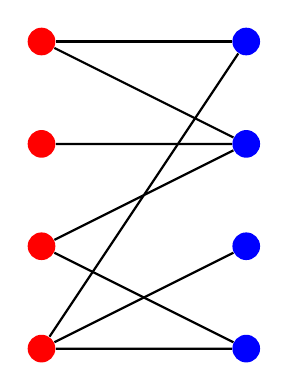
\begin{tikzpicture}[scale=1.3,auto,swap]
  \node[red vertex] (a) at (0,0) {};
  \node[blue vertex] (b) at (2,0) {};
  \node[blue vertex] (c) at (2,-1) {};
  \node[red vertex] (d) at (0,-1) {};
  \node[red vertex] (e) at (0,-2) {};
  \node[red vertex] (f) at (0,-3) {};
  \node[blue vertex] (g) at (2,-2) {};
  \node[blue vertex] (h) at (2,-3) {};
  \draw[edge] (a) to (b);
  \draw[edge] (a) to (c);
  \draw[edge] (b) to (f);
  \draw[edge] (c) to (d);
  \draw[edge] (c) to (e);
  \draw[edge] (f) to (h);
  \draw[edge] (e) to (h);
  \draw[edge] (f) to (g);
\end{tikzpicture}

      \end{center}
      \vspace{0.1cm}
    \end{exampleblock}}
  \end{columns}
\end{frame}

\section{Articulation Points}
\begin{frame}
  \begin{center}
    {\bf Part III -- Articulation Vertices and Edges}
  \end{center}
\end{frame}

\begin{frame}
  \frametitle{Articulation Points and Bridges}
    \begin{block}{Definition: In a graph $G$}
      \begin{itemize}
      \item Vertex $v_i$ is an {\bf Articulation Point} if removing $v_i$ makes $G$ disconnected.
      \item Edge $e_{i,j}$ is a {\bf Bridge} if removing $e_{i,j}$ makes $G$ disconnected.
      \end{itemize}
    \end{block}
    \begin{center}
        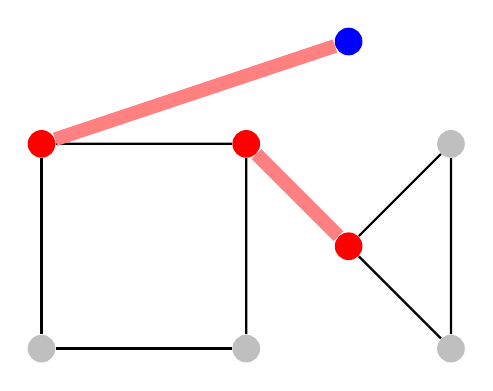
\begin{tikzpicture}[scale=1.3,auto,swap]
          \node[vertex] (a) at (0,0) {};
          \node[vertex] (b) at (2,0) {};
          \node[red vertex] (c) at (0,2) {};
          \node[red vertex] (d) at (2,2) {};
          \node[red vertex] (e) at (3,1) {};
          \node[vertex] (f) at (4,0) {};
          \node[vertex] (g) at (4,2) {};
          \node[blue vertex] (h) at (3,3) {};
          \draw[edge] (a) to (b);
          \draw[edge] (a) to (c);
          \draw[edge] (c) to (d);
          \draw[edge] (d) to (b);
          \draw[red edge] (d) to (e);
          \draw[edge] (e) to (f);
          \draw[edge] (f) to (g);
          \draw[edge] (g) to (e);
          \draw[red edge] (c) to (h);
        \end{tikzpicture}
      \end{center}
\end{frame}

\begin{frame}
  \frametitle{Problems and Naive Algorithm}
  \begin{exampleblock}{Example Problems}
    \begin{itemize}
      \item Find vertices that can be removed from a graph to "break" it;
      \item Add extra edges to "reinforce" a graph;
      \item Measure the reliability of a network, etc;
    \end{itemize}
  \end{exampleblock}\medskip

  \begin{block}{Complete Search algorithm to find Articulation Points: $O(V\times(V+E)) = O(V^2+VE)$}
  \begin{enumerate}
    \item Run DFS/BFS, and count the number of CC in the graph;
    \item For each vertex $v_i$, remove $v_i$ and run DFS/BFS again;
    \item If the number of CC increases, $v_i$ is an articulation point;
  \end{enumerate}
  \end{block}
\end{frame}

\begin{frame}{Tarjan's DFS variant for Articulation point (O(V+E))}
  \begin{exampleblock}{Find Articulation Points/Bridges in a single DFS pass: $O(V+E)$}
    Main idea: Track loops to detect articulations:
    \begin{itemize}
    \item {\bf dfs\_num[i]}: visitation order from DFS;
    \item {\bf dfs\_low[i]}: lowest dfs\_num reachable from $v_i$;
    \end{itemize}\bigskip

    For neighbors $u,v$, if low[$v$] >= num[$u$], then $u$ is an articulation node (except root)\bigskip

    For neighbors $u,v$, if low[$v$] > num[$u$], $e_{u,v}$ is a bridge; (articulation edge)
  \end{exampleblock}
\end{frame}

% \begin{frame}{Tarjan's DFS variant for Articulation point (O(V+E))}
%
%   \begin{center}
%     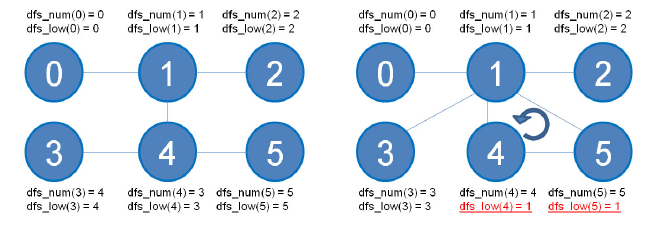
\includegraphics[width=0.9\textwidth]{../img/graph_articulation}
%   \end{center}
%   \ppagenote{Tarjan's attributes image from Competitive Programming 3}
% \end{frame}

\begin{frame}{Tarjan's Algorithm for Articulation Point}{Simulation}
  \begin{columns}
    \column{.45\textwidth}
    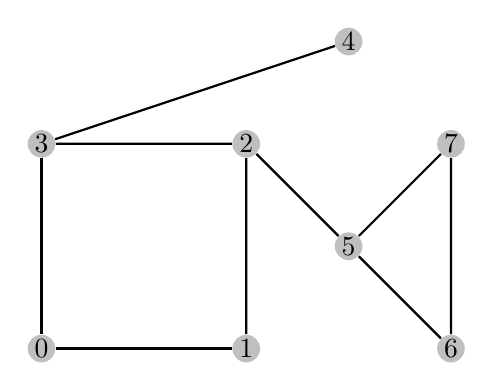
\begin{tikzpicture}[scale=1.3,auto,swap]
      \node[vertex] (a) at (0,0) {0};
      \node[vertex] (b) at (2,0) {1};
      \node[vertex] (c) at (0,2) {3};
      \node[vertex] (d) at (2,2) {2};
      \node[vertex] (e) at (3,1) {5};
      \node[vertex] (f) at (4,0) {6};
      \node[vertex] (g) at (4,2) {7};
      \node[vertex] (h) at (3,3) {4};
      \draw[edge] (a) to (b);
      \draw[edge] (a) to (c);
      \draw[edge] (c) to (d);
      \draw[edge] (d) to (b);
      \draw[edge] (d) to (e);
      \draw[edge] (e) to (f);
      \draw[edge] (f) to (g);
      \draw[edge] (g) to (e);
      \draw[edge] (c) to (h);
    \end{tikzpicture}
    \column{.55\textwidth}
    First, use DFS to calculate dfs\_num and dfs\_low\\
    Then compare neighbors to check articulation node/edge.
    \begin{itemize}
      \item dfs\_num: 0; dfs\_low: 0
      \item dfs\_num: 1; dfs\_low: 0
      \item dfs\_num: 2; dfs\_low: 0
      \item dfs\_num: 3; dfs\_low: 0
      \item dfs\_num: 4; dfs\_low: 4
      \item dfs\_num: 5; dfs\_low: 5
      \item dfs\_num: 6; dfs\_low: 5
      \item dfs\_num: 7; dfs\_low: 5
    \end{itemize}
  \end{columns}
\end{frame}

\begin{frame}[fragile]{Tarjan's Algorithm for Articulation Point}
  
{\smaller
  \begin{exampleblock}{}
\begin{verbatim}
void articulation(u){
   dfs_num[u] = dfs_low[u] = IterationCounter++; // update num[u], init low[u]
   for (int i = 0; i < AdjList[u].size(); i++){  // Do DFS on each edge from u
      v = AdjList[u][i];
      if (dfs_num[v.first] == UNVISITED) {       // DFS tree edge
         dfs_parent[v.first] = u;                // store parent
         if (u == 0) rootTreeEdge++;             // special case for root vertex
         articulation(v.first);                  // visit next vertex

         // After we finish the DFS from u, we check if u is articulation.
         if (dfs_low[v.first] >= dfs_num[u])
            articulation_vertex[u] = true;       // u is articulation
         dfs_low[u] = min(dfs_low[u],dfs_low[v.first])
      }
      else if (v.first != dfs_parent[u])         // found a cycle edge
         dfs_low[u] = min(dfs_low[u],dfs_num[v.first]);
}  }
\end{verbatim}
  \end{exampleblock}}
\end{frame}

\subsection{Strongly Connected Components}

\begin{frame}{Strongly Connected Components}
    \begin{block}{Definition}
      Given a {\bf directed} graph $G(V,E)$, a {\bf Strongly Connected Component (SCC)} is a subset of vertices $V_1$ where for every pair of vertices $v_i, v_j \in V_1$, there is both a path $v_i \to v_j$ and a path $v_j \to v_i$.
    \end{block}


\begin{columns}[t]
    \column{0.5\textwidth}
    \begin{exampleblock}{One Connected Component (undirected)}
      \vspace{0.1cm}
      \begin{center}
        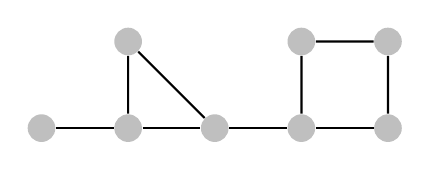
\begin{tikzpicture}[scale=1.1,auto,swap]
          \node[vertex] (a) at (0,0) {};
          \node[vertex] (b) at (1,0) {};
          \node[vertex] (c) at (2,0) {};
          \node[vertex] (d) at (1,1) {};
          \node[vertex] (e) at (3,0) {};
          \node[vertex] (f) at (4,0) {};
          \node[vertex] (g) at (4,1) {};
          \node[vertex] (h) at (3,1) {};
          \draw[edge] (a) to (b);
          \draw[edge] (b) to (c);
          \draw[edge] (c) to (d);
          \draw[edge] (d) to (b);
          \draw[edge] (c) to (e);
          \draw[edge] (e) to (f);
          \draw[edge] (f) to (g);
          \draw[edge] (g) to (h);
          \draw[edge] (h) to (e);
        \end{tikzpicture}
      \end{center}
      \vspace{0.1cm}
    \end{exampleblock}
    \column{0.5\textwidth}
    \begin{exampleblock}{Three SCC (directed)}
      \vspace{0.1cm}
      \begin{center}
        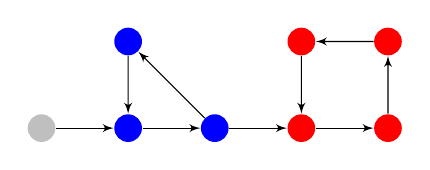
\begin{tikzpicture}[scale=1.1,auto,swap]
          \tikzset{edge/.style = {->,>=latex'}}
          \node[vertex] (a) at (0,0) {};
          \node[blue vertex] (b) at (1,0) {};
          \node[blue vertex] (c) at (2,0) {};
          \node[blue vertex] (d) at (1,1) {};
          \node[red vertex] (e) at (3,0) {};
          \node[red vertex] (f) at (4,0) {};
          \node[red vertex] (g) at (4,1) {};
          \node[red vertex] (h) at (3,1) {};
          \draw[edge] (a) to (b);
          \draw[edge] (b) to (c);
          \draw[edge] (c) to (d);
          \draw[edge] (d) to (b);
          \draw[edge] (c) to (e);
          \draw[edge] (e) to (f);
          \draw[edge] (f) to (g);
          \draw[edge] (g) to (h);
          \draw[edge] (h) to (e);
        \end{tikzpicture}
      \end{center}
      \vspace{0.1cm}
    \end{exampleblock}
  \end{columns}
\end{frame}

\begin{frame}{Algorithm for Finding SCCs}

  We can modify Tarjan's algorithm (for articulation points and bridges) to find Strongly Connected Components:\bigskip

  \begin{block}{}
  \begin{itemize}
    \item Every time we visit a new vertex $u$, we put $u$ in a stack $S$;
    \item Only update dfs\_low for vertices with the "visited" flag = 1;
    \item After visiting all edges of $u$, check if "dfs\_num[$u$] == dfs\_low[$u$]";
    \item If the condition is true, $u$ is the root of a new SCC.
    \item Pop all vertices in $S$ until (and including) $u$;
    \item Add all popped vertices to the SCC.
  \end{itemize}
  \end{block}
\end{frame}

\begin{frame}[fragile]{Algorithm for Finding SCCs}{Do this simulation yourself!}
  \begin{center}
    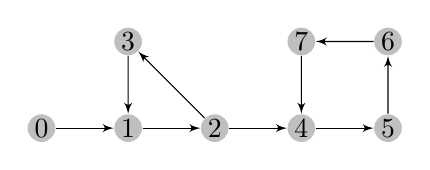
\begin{tikzpicture}[scale=1.1,auto,swap]
      \tikzset{edge/.style = {->,>=latex'}}
      \node[vertex] (a) at (0,0) {0};
      \node[vertex] (b) at (1,0) {1};
      \node[vertex] (c) at (2,0) {2};
      \node[vertex] (d) at (1,1) {3};
      \node[vertex] (e) at (3,0) {4};
      \node[vertex] (f) at (4,0) {5};
      \node[vertex] (g) at (4,1) {6};
      \node[vertex] (h) at (3,1) {7};
      \draw[edge] (a) to (b);
      \draw[edge] (b) to (c);
      \draw[edge] (c) to (d);
      \draw[edge] (d) to (b);
      \draw[edge] (c) to (e);
      \draw[edge] (e) to (f);
      \draw[edge] (f) to (g);
      \draw[edge] (g) to (h);
      \draw[edge] (h) to (e);
    \end{tikzpicture}
  \end{center}
  \bigskip
  {\bf SCC Stack:}\bigskip

\begin{verbatim}
          0   1   2   3   4   5   6   7

dfs_low

dfs_num
\end{verbatim}

\end{frame}

%%%%%%%%%%%%%%%%%%%%%%%%%%%%%%%%%%%%%%%%%%%%%%%

\begin{frame}
  \begin{center}
    {\bf Part 4: Minimum Spanning Tree}
  \end{center}
\end{frame}

\subsection{Spanning Tree}
\begin{frame}
  \frametitle{Minimum Spanning Trees (MST) -- Definition}

  \begin{block}{}
    A {\bf Spanning Tree} is a subset $E'$ from graph $G$ so
    that all vertices are connected without cycles.

    \medskip

    A \structure{Minimum Spanning Tree} is a spanning tree where the
    sum of edge's weights is minimal.
  \end{block}

  \begin{columns}[T]
    Graph\\
    \column{0.3\textwidth}
    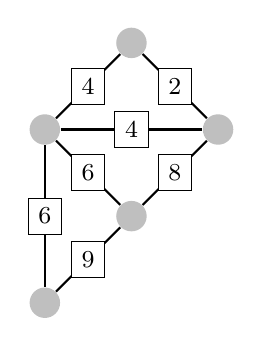
\begin{tikzpicture}[transform shape,label/.style={thin, draw=black, align=center,fill=white,font=\smaller},scale=1.1]
      \node[vertex] (a) at (0,0) {};
      \node[vertex] (b) at (1,1) {};
      \node[vertex] (c) at (2,0) {};
      \node[vertex] (d) at (1,-1) {};
      \node[vertex] (e) at (0,-2) {};
      \draw[edge] (a) -- node[label] {$4$} (b);
      \draw[edge] (b) -- node[label] {$2$} (c);
      \draw[edge] (a) -- node[label] {$4$} (c);
      \draw[edge] (a) -- node[label] {$6$} (d);
      \draw[edge] (c) -- node[label] {$8$} (d);
      \draw[edge] (a) -- node[label] {$6$} (e);
      \draw[edge] (d) -- node[label] {$9$} (e);
    \end{tikzpicture}
    \column{0.3\textwidth}
    Spanning Tree
    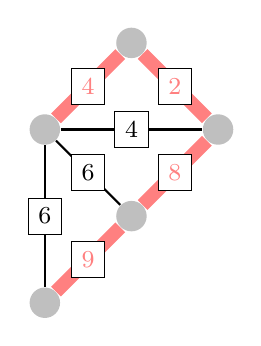
\begin{tikzpicture}[transform shape,label/.style={thin, draw=black, align=center,fill=white,font=\smaller},scale=1.1]
      \node[vertex] (a) at (0,0) {};
      \node[vertex] (b) at (1,1) {};
      \node[vertex] (c) at (2,0) {};
      \node[vertex] (d) at (1,-1) {};
      \node[vertex] (e) at (0,-2) {};
      \draw[red edge] (a) -- node[label] {$4$} (b);
      \draw[red edge] (b) -- node[label] {$2$} (c);
      \draw[edge] (a) -- node[label] {$4$} (c);
      \draw[edge] (a) -- node[label] {$6$} (d);
      \draw[red edge] (c) -- node[label] {$8$} (d);
      \draw[edge] (a) -- node[label] {$6$} (e);
      \draw[red edge] (d) -- node[label] {$9$} (e);
    \end{tikzpicture}
    \column{0.3\textwidth}
    Minimum Spanning Tree
    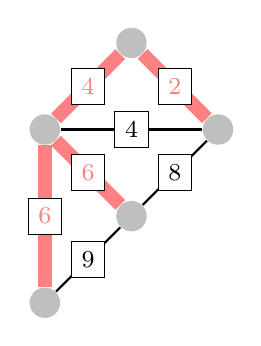
\begin{tikzpicture}[transform shape,label/.style={thin, draw=black, align=center,fill=white,font=\smaller},scale=1.1]
      \node[vertex] (a) at (0,0) {};
      \node[vertex] (b) at (1,1) {};
      \node[vertex] (c) at (2,0) {};
      \node[vertex] (d) at (1,-1) {};
      \node[vertex] (e) at (0,-2) {};
      \draw[red edge] (a) -- node[label] {$4$} (b);
      \draw[red edge] (b) -- node[label] {$2$} (c);
      \draw[edge] (a) -- node[label] {$4$} (c);
      \draw[red edge] (a) -- node[label] {$6$} (d);
      \draw[edge] (c) -- node[label] {$8$} (d);
      \draw[red edge] (a) -- node[label] {$6$} (e);
      \draw[edge] (d) -- node[label] {$9$} (e);
    \end{tikzpicture}
  \end{columns}
\end{frame}

\begin{frame}{Usage Cases for Minimum Spanning Trees}
  \begin{block}{}
    \begin{itemize}
      \item Problems with MST often ask for a minimal cost to connect all elements in a graph (e.g. minimal infrastructure cost).\medskip

      \item {\bf Variations:} Maximum Spanning Tree, Spanning Forest, Force some edges in advance;
    \end{itemize}
  \end{block}

  \begin{exampleblock}{Main algorithms for MST}
    Two greedy algorithms that add edges to MST:
    \begin{itemize}
      \item {\bf Kruskal Algorithm}: based on edge list;
      \item {\bf Prim's Algorithm}: based on vertex list;
    \end{itemize}
  \end{exampleblock}
\end{frame}

\begin{frame}
  \frametitle{Kruskal's Algorithm}
  \begin{block}{Outline}
    Kruskal's algorithms sorts all edges by their weight, and try to add each edge to the MST, checking whether adding that edge would create a cycle.
  \end{block}

  \begin{columns}[T]
    \column{0.5\textwidth}
    \begin{enumerate}
    \item Sort all edges;
    \item If smallest edge does not create a cycle, add to MST;
    \item If smallest edge creates a cycle, remove it from list;
    \item Go to 2;
    \end{enumerate}
    \column{0.5\textwidth}
    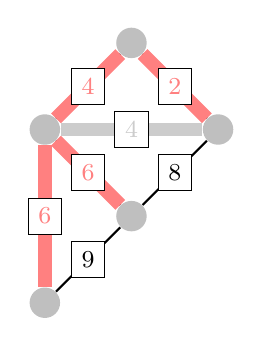
\begin{tikzpicture}[transform shape,label/.style={thin, draw=black, align=center,fill=white,font=\smaller},scale=1.1]
      \node[vertex] (a) at (0,0) {};
      \node[vertex] (b) at (1,1) {};
      \node[vertex] (c) at (2,0) {};
      \node[vertex] (d) at (1,-1) {};
      \node[vertex] (e) at (0,-2) {};
      \draw[edge] (a) -- node[label] {$4$} (b);
      \draw[edge] (b) -- node[label] {$2$} (c);
      \draw[edge] (a) -- node[label] {$4$} (c);
      \draw[edge] (a) -- node[label] {$6$} (d);
      \draw[edge] (c) -- node[label] {$8$} (d);
      \draw[edge] (a) -- node[label] {$6$} (e);
      \draw[edge] (d) -- node[label] {$9$} (e);
      \draw<2->[red edge] (b) -- node[label] {$2$} (c);
      \draw<3->[red edge] (a) -- node[label] {$4$} (b);
      \draw<4->[black edge] (a) -- node[label] {$4$} (c);
      \draw<4->[red edge] (a) -- node[label] {$6$} (d);
      \draw<5->[red edge] (a) -- node[label] {$6$} (e);
    \end{tikzpicture}
  \end{columns}
\end{frame}

\begin{frame}[fragile]
  \frametitle{Kruskal's Algorithm -- Implementation}
{\smaller
\begin{exampleblock}{}
\begin{verbatim}
vector<pair<int, pair<int,int>> Edgelist;
sort(Edgelist.begin(),Edgelist.end());
int mst_cost = 0;
UnionFind UF(V);
  // note 1: Pair object has built-in comparison;
  // note 2: Need to implement UnionSet class;

for (int i = 0; i < Edgelist.size(); i++) {
   pair <int, pair <int,int>> front = Edgelist[i];
   if (!UF.isSameSet(front.second.first,
                     front.second.second)) {
      mst_cost += front.first;
      UF.unionSet(front.second.first,front.second.second)
   }}

cout << "MST Cost: " << mst_cost << "\n"
\end{verbatim}
\end{exampleblock}
}
\end{frame}

\begin{frame}
  \frametitle{Prim's Algorithm}
  {\small
  \begin{block}{Outline}
    Prim's algorith adds nodes to the MST one at a time, and keeps the
    edges connected to those nodes in a \structure{priority queue}. It
    then tests each edge in the priority queue to add more nodes to
    the MST, avoiding cycles.
  \end{block}

  \begin{columns}[T]
    \column{0.5\textwidth}
    \begin{enumerate}
    \item Add node 0 to MST;
    \item Add all edges from new node to Priority Queue;
    \item Visit smallest edge in Queue;
    \item If the edge leades to a new node, add it to MST;
    \item Add new edges to Queue;
    \item Go to 3;
    \end{enumerate}
    \column{0.5\textwidth}
    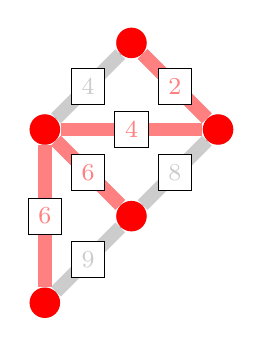
\begin{tikzpicture}[transform shape,label/.style={thin, draw=black, align=center,fill=white,font=\smaller},scale=1.1]
      \node[vertex] (a) at (0,0) {};
      \node[vertex] (b) at (1,1) {};
      \node[vertex] (c) at (2,0) {};
      \node[vertex] (d) at (1,-1) {};
      \node[vertex] (e) at (0,-2) {};
      \draw[edge] (a) -- node[label] {$4$} (b);
      \draw[edge] (b) -- node[label] {$2$} (c);
      \draw[edge] (a) -- node[label] {$4$} (c);
      \draw[edge] (a) -- node[label] {$6$} (d);
      \draw[edge] (c) -- node[label] {$8$} (d);
      \draw[edge] (a) -- node[label] {$6$} (e);
      \draw[edge] (d) -- node[label] {$9$} (e);
      \uncover<2->{
      \node[red vertex] (a1) at (0,0) {};
      \draw[black edge] (a) -- node[label] {$4$} (b);
      \draw[black edge] (a) -- node[label] {$4$} (c);
      \draw[black edge] (a) -- node[label] {$6$} (d);
      \draw[black edge] (a) -- node[label] {$6$} (e);
      }

      \uncover<3->{
        \node[red vertex] (c1) at (2,0) {};
        \draw[red edge] (a) -- node[label] {$4$} (c);
        \draw[black edge] (c) -- node[label] {$8$} (d);
        \draw[black edge] (b) -- node[label] {$2$} (c);
      }
      \uncover<4->{
        \node[red vertex] (b1) at (1,1) {};
        \draw[red edge] (b) -- node[label] {$2$} (c);
      }

      \uncover<5->{
        \node[red vertex] (d1) at (1,-1) {};
        \draw[red edge] (a) -- node[label] {$6$} (d);
        \draw[black edge] (d) -- node[label] {$9$} (e);
      }

      \uncover<6->{
        \node[red vertex] (e1) at (0,-2) {};
        \draw[red edge] (a) -- node[label] {$6$} (e);
      }
    \end{tikzpicture}
  \end{columns}
  }
\end{frame}

\begin{frame}[fragile]
  \frametitle{Prim's Algorithm -- Implementation}
{\smaller
\begin{exampleblock}{}
\begin{verbatim}
vector <int> taken; priority_queue <pair <int,int>> pq;

void process (int v) {
   taken[v] = 1;
   for (int j = 0; j < (int)AdjList[v].size(); j++) {
      pair <int,int> ve = AdjList[v][j];
      if (!taken[ve.first])
         pq.push(pair <int,int> (ve.first, ve.second))
}}
taken.assign(V,0); process(0);
mst_cost = 0;

while (!pq.empty()) {
  vector <int,int> pq.top(); pq.pop();
  u = front.first, w = front.second;
  if (!taken[u]) mst_cost += w, process(u);
}
\end{verbatim}
\end{exampleblock}
}
\end{frame}

\begin{frame}
  \frametitle{MST variant 1 -- Maximum Spanning tree}

    \begin{block}{}
      The \structure{Maximum Spanning Tree} variant requires the spanning tree to have maximum possible weight.\bigskip


      It is very easy to implement the Maximum MST:
      \begin{itemize}
        \item {\bf Kruskal}: Reverse the sort of the edge list;
        \item {\bf Prim}: Invert the weight of the priority queue;
      \end{itemize}
    \end{block}

  \medskip

  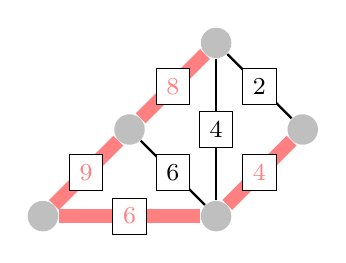
\begin{tikzpicture}[transform shape,label/.style={thin, draw=black, align=center,fill=white,font=\smaller},scale=1.1]
      \node[vertex] (a) at (0,0) {};
      \node[vertex] (b) at (1,1) {};
      \node[vertex] (c) at (0,2) {};
      \node[vertex] (d) at (-1,1) {};
      \node[vertex] (e) at (-2,0) {};
      \draw[red edge] (a) -- node[label] {$4$} (b);
      \draw[edge] (b) -- node[label] {$2$} (c);
      \draw[edge] (a) -- node[label] {$4$} (c);
      \draw[edge] (a) -- node[label] {$6$} (d);
      \draw[red edge] (c) -- node[label] {$8$} (d);
      \draw[red edge] (a) -- node[label] {$6$} (e);
      \draw[red edge] (d) -- node[label] {$9$} (e);
  \end{tikzpicture}
\end{frame}

\begin{frame}
  \frametitle{MST variant 2 -- Minimum Spanning Subgraph, Forest}
    \begin{block}{}
      In this variant, a subset of edges or vertices are pre-selected.

      \begin{itemize}
      \item In the case of pre-selected vertices, add them to the
        ``taken'' list in Kruskal's algorithm before starting;
      \item In the case of edges, add the end vertices to the
        ``taken'' list;
      \end{itemize}
    \end{block}\bigskip

    \begin{center}
      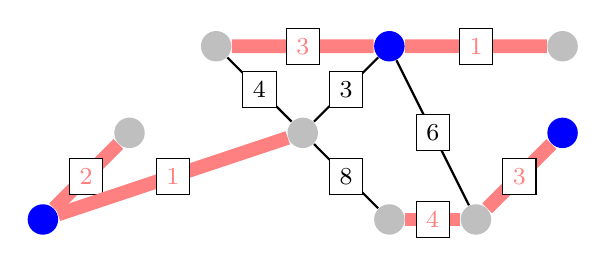
\begin{tikzpicture}[transform shape,label/.style={thin, draw=black, align=center,fill=white,font=\smaller},scale=1.1]
        \node[blue vertex] (a) at (0,0) {};
        \node[vertex] (b) at (1,1) {};
        \node[vertex] (c) at (2,2) {};
        \node[vertex] (d) at (3,1) {};
        \node[vertex] (e) at (4,0) {};
        \node[blue vertex] (f) at (4,2) {};
        \node[vertex] (g) at (5,0) {};
        \node[vertex] (h) at (6,2) {};
        \node[blue vertex] (i) at (6,1) {};
        \draw[red edge] (a) -- node[label] {$2$} (b);
        \draw[red edge] (a) -- node[label] {$1$} (d);
        \draw[edge] (d) -- node[label] {$4$} (c);
        \draw[edge] (d) -- node[label] {$8$} (e);
        \draw[edge] (d) -- node[label] {$3$} (f);
        \draw[red edge] (c) -- node[label] {$3$} (f);
        \draw[edge] (f) -- node[label] {$6$} (g);
        \draw[red edge] (e) -- node[label] {$4$} (g);
        \draw[red edge] (f) -- node[label] {$1$} (h);
        \draw[red edge] (g) -- node[label] {$3$} (i);
      \end{tikzpicture}
    \end{center}
\end{frame}

\begin{frame}
  \frametitle{MST Variant 3 -- Second Best MST}
  \begin{block}{Problem Definition}
    Suppose that you are required to calculate an alternative solution to an MST problem. In this case, you need to find the second cheapest spanning tree.
  \end{block}
  \bigskip

  Simple Algorithm:
  \begin{itemize}
    \item Calculate the MST (using Kruskal or Prim);
    \item For every edge $e_i$ in the MST:
    \begin{itemize}
      \item Remove $e_i$ from $E$;
      \item Calculate a new MST;
    \end{itemize}
    \item Choose the best among the new MSTs as the second-best MST.
  \end{itemize}
  \bigskip

  {\bf QUIZ}: How to generalize this algorithm for the n-th best spanning tree?
\end{frame}

\begin{frame}
  \frametitle{MST Variant 4 -- Minmax path cost}

  \begin{center}
      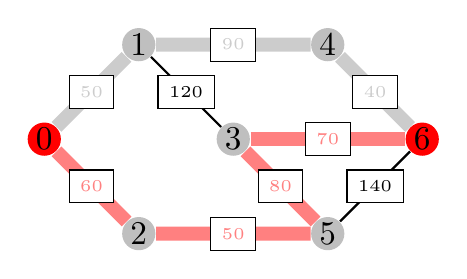
\begin{tikzpicture}[transform shape,label/.style={thin, draw=black, align=center,fill=white,font=\tiny},scale=1.2]
        \node[red vertex] (a) at (0,0) {0};
        \node[vertex] (b) at (1,1) {1};
        \node[vertex] (c) at (1,-1) {2};
        \node[vertex] (d) at (2,0) {3};
        \node[vertex] (e) at (3,1) {4};
        \node[vertex] (f) at (3,-1) {5};
        \node[red vertex] (g) at (4,0) {6};
        \draw[black edge] (a) -- node[label] {$50$} (b);
        \draw[red edge] (a) -- node[label] {$60$} (c);
        \draw[edge] (b) -- node[label] {$120$} (d);
        \draw[black edge] (b) -- node[label] {$90$} (e);
        \draw[red edge] (c) -- node[label] {$50$} (f);
        \draw[red edge] (d) -- node[label] {$80$} (f);
        \draw[red edge] (d) -- node[label] {$70$} (g);
        \draw[black edge] (e) -- node[label] {$40$} (g);
        \draw[edge] (f) -- node[label] {$140$} (g);
      \end{tikzpicture}
    \end{center}

  \begin{block}{Problem Definition}
    {\bf Regular Cost} for a path is the sum of weights of all edges in the path.\bigskip

    {\bf Minmax Cost} for a path is the maximum weight among all its edges.\bigskip

    Find the path $v_i \to v_j$ with the smallest {\bf minmax cost}
  \end{block}
\end{frame}

\begin{frame}
  \frametitle{Finding the Minmax path with MST}

  \begin{center}
      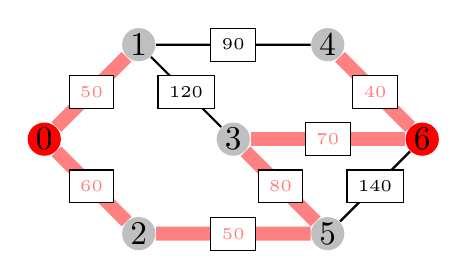
\begin{tikzpicture}[transform shape,label/.style={thin, draw=black, align=center,fill=white,font=\tiny},scale=1.2]
        \node[red vertex] (a) at (0,0) {0};
        \node[vertex] (b) at (1,1) {1};
        \node[vertex] (c) at (1,-1) {2};
        \node[vertex] (d) at (2,0) {3};
        \node[vertex] (e) at (3,1) {4};
        \node[vertex] (f) at (3,-1) {5};
        \node[red vertex] (g) at (4,0) {6};
        \draw[red edge] (a) -- node[label] {$50$} (b);
        \draw[red edge] (a) -- node[label] {$60$} (c);
        \draw[edge] (b) -- node[label] {$120$} (d);
        \draw[edge] (b) -- node[label] {$90$} (e);
        \draw[red edge] (c) -- node[label] {$50$} (f);
        \draw[red edge] (d) -- node[label] {$80$} (f);
        \draw[red edge] (d) -- node[label] {$70$} (g);
        \draw[red edge] (e) -- node[label] {$40$} (g);
        \draw[edge] (f) -- node[label] {$140$} (g);
      \end{tikzpicture}
    \end{center}

  \begin{exampleblock}{Algorithm}
    \begin{itemize}
      \item Generate the MST for the graph $G$.
      \item Find the path $v_i \to v_j$ inside the MST.
    \end{itemize}\bigskip

    That's it!
  \end{exampleblock}
\end{frame}


%%%%%%%%%%%%%%%%%%%%%%%%%%%%%%%%%%%%%%%%%%%%%%%%%%%%
\section{Backmatter}
\begin{frame}{About these Slides}
  These slides were made by Claus Aranha, 2020. You are welcome to copy, re-use and modify this material.
  \bigskip

  Individual images in some slides might have been made by other
  authors. Please see the references in each slide for those cases.
\end{frame}

\begin{frame}[allowframebreaks]{Image Credits}
  \printnotes
\end{frame}

\end{CJK}
\end{document}
